\contribution{A Brief Introduction }
\shortcontributor{CS6230 : CAD for VLSI Project Report}
\shortcontribution{Vector Extensions}
\headnum{5}
\begin{paper}
\renewcommand*{\pagemark}{}
\section*{}
\begin{figure}[H]
\centering
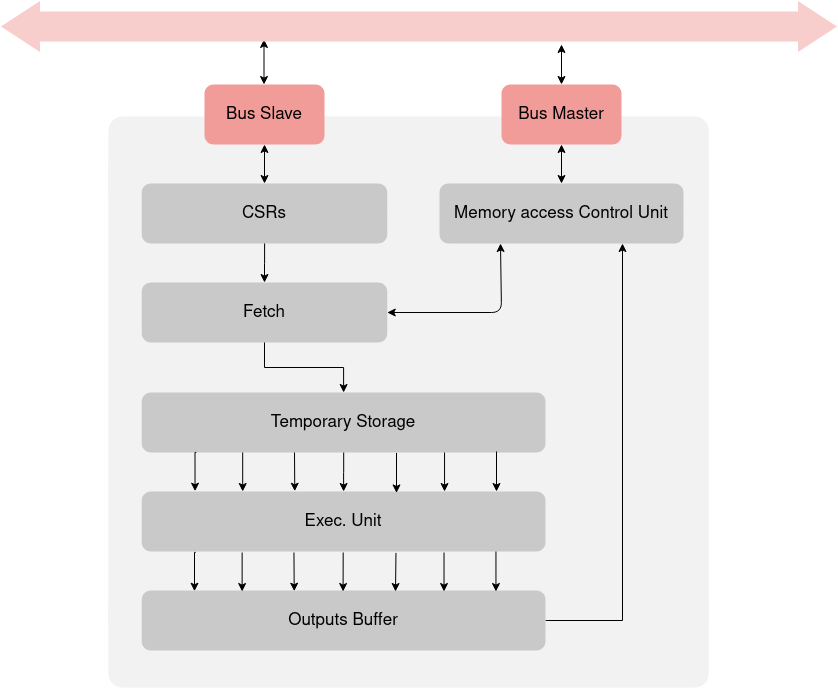
\includegraphics[width=11cm]{Images/VectorExtensions.png}
\caption{\content General architecture of our Vector Processing Unit.}
\end{figure}\\
\nointend The general architecture for a vector accelerator is as given in the figure. While such a formation is suitable for most vector operations, matrix operations may require a
different kind of design with systolic arrays. Since we intend to devise a design for accelerators concerning vector negation and statistics minimum, we restrict the general design for vector operations. It is to be remarked that slight alterations in dataflow may be required for binary vector operations.\\\\
\nointend The CPU writes the pointers for the source & destination vectors and the vector size into the accelerators' CSRs. Once the CPU instructs the accelerator to start computation by writing to the start flag of the CSRs, the fetch unit requests the memory access controller for the data. The memory access controller handles read/write requests and responses between the accelerator and the bus. The memory access controller uses round-robin scheduling for handling simultaneous read and write requests. Once the fetch unit gets the data corresponding to a portion of the vector, it gets enqueued onto the temporary storage unit.

\end{paper}